%TOASK
%---------------------------------------------------------------------
%   documentclass
%---------------------------------------------------------------------
\documentclass[]{beamer}
% Class options include: notes, notesonly, handout, trans,
%                        hidesubsections, shadesubsections,
%                        inrow, blue, red, grey, brown

%---------------------------------------------------------------------
%   packages
%---------------------------------------------------------------------
% Theme for beamer presentation.
\usepackage{beamerthemesplit}
% Other themes include: beamerthemebars, beamerthemelined,
%                       beamerthemetree, beamerthemetreebars
\usepackage[english]{babel}
\usepackage[enc=cp1250]{hrlatex}
\usepackage[T1]{fontenc} %pekne makcene
\usepackage{lmodern} %spolu s T1 smooth font!
\usepackage{tikz}
\usepackage{cite} %bibtex
\usepackage[numbers]{natbib}
\usepackage{color} %for \textcolor{declared-color}{text}
\usepackage{floatflt} %to have tables and text beside
\usepackage{colortbl} %for \rowcolor command
\usepackage{scalefnt} %for scale font
\usepackage{pifont} %for ticks (check symbols)
\usetikzlibrary{decorations.pathreplacing}

%---------------------------------------------------------------------
%   settings
%---------------------------------------------------------------------
\graphicspath{{./pics/}} %picture dir

\definecolor{tablehead}{RGB}{238,233,233} %nice smooth grey

\def\Tiny{ \font\Tinyfont = cmr10 at 3pt \relax  \Tinyfont}

\pgfrealjobname{presentation} % <-- NOTE: this needs to be the real document's basename
                        %     (else you'll only get an empty output file)

\newif\iffull
\fullfalse

\newif\iffinal % introduce a switch for draft vs. final document
\finaltrue % use this to compile the final document
\iffinal
  \newcommand{\inputTikZ}[1]{%
    \input{#1.tikz}%
  }
\else
  \newcommand{\inputTikZ}[1]{%
    \beginpgfgraphicnamed{#1-external}%
    \input{#1.tikz}%
    \endpgfgraphicnamed%
  }
\fi

%---------------------------------------------------------------------
%   environments
%---------------------------------------------------------------------
%\newcommand{\newblock}{}

\newcommand{\tick}{\ding{52}}
\newcommand{\cross}{\ding{55}}

%---------------------------------------------------------------------
%   theme
%---------------------------------------------------------------------
\usetheme{Darmstadt}
\usecolortheme{crane}

%---------------------------------------------------------------------
%   data
%---------------------------------------------------------------------
\title{\textbf{Oracles for timetable graphs}}
\subtitle{Or�kula pre grafy reprezentuj�ce cestovn� poriadky}
\author{\textbf{Franti�ek Hajnovi�}}
\institute{FMFI UK}
\date{\today}

%---------------------------------------------------------------------
%   document
%---------------------------------------------------------------------
\begin{document}

	%---------------------------------------------------------------------
	%   Title page
	%---------------------------------------------------------------------
	{
    \setbeamertemplate{background canvas}{
        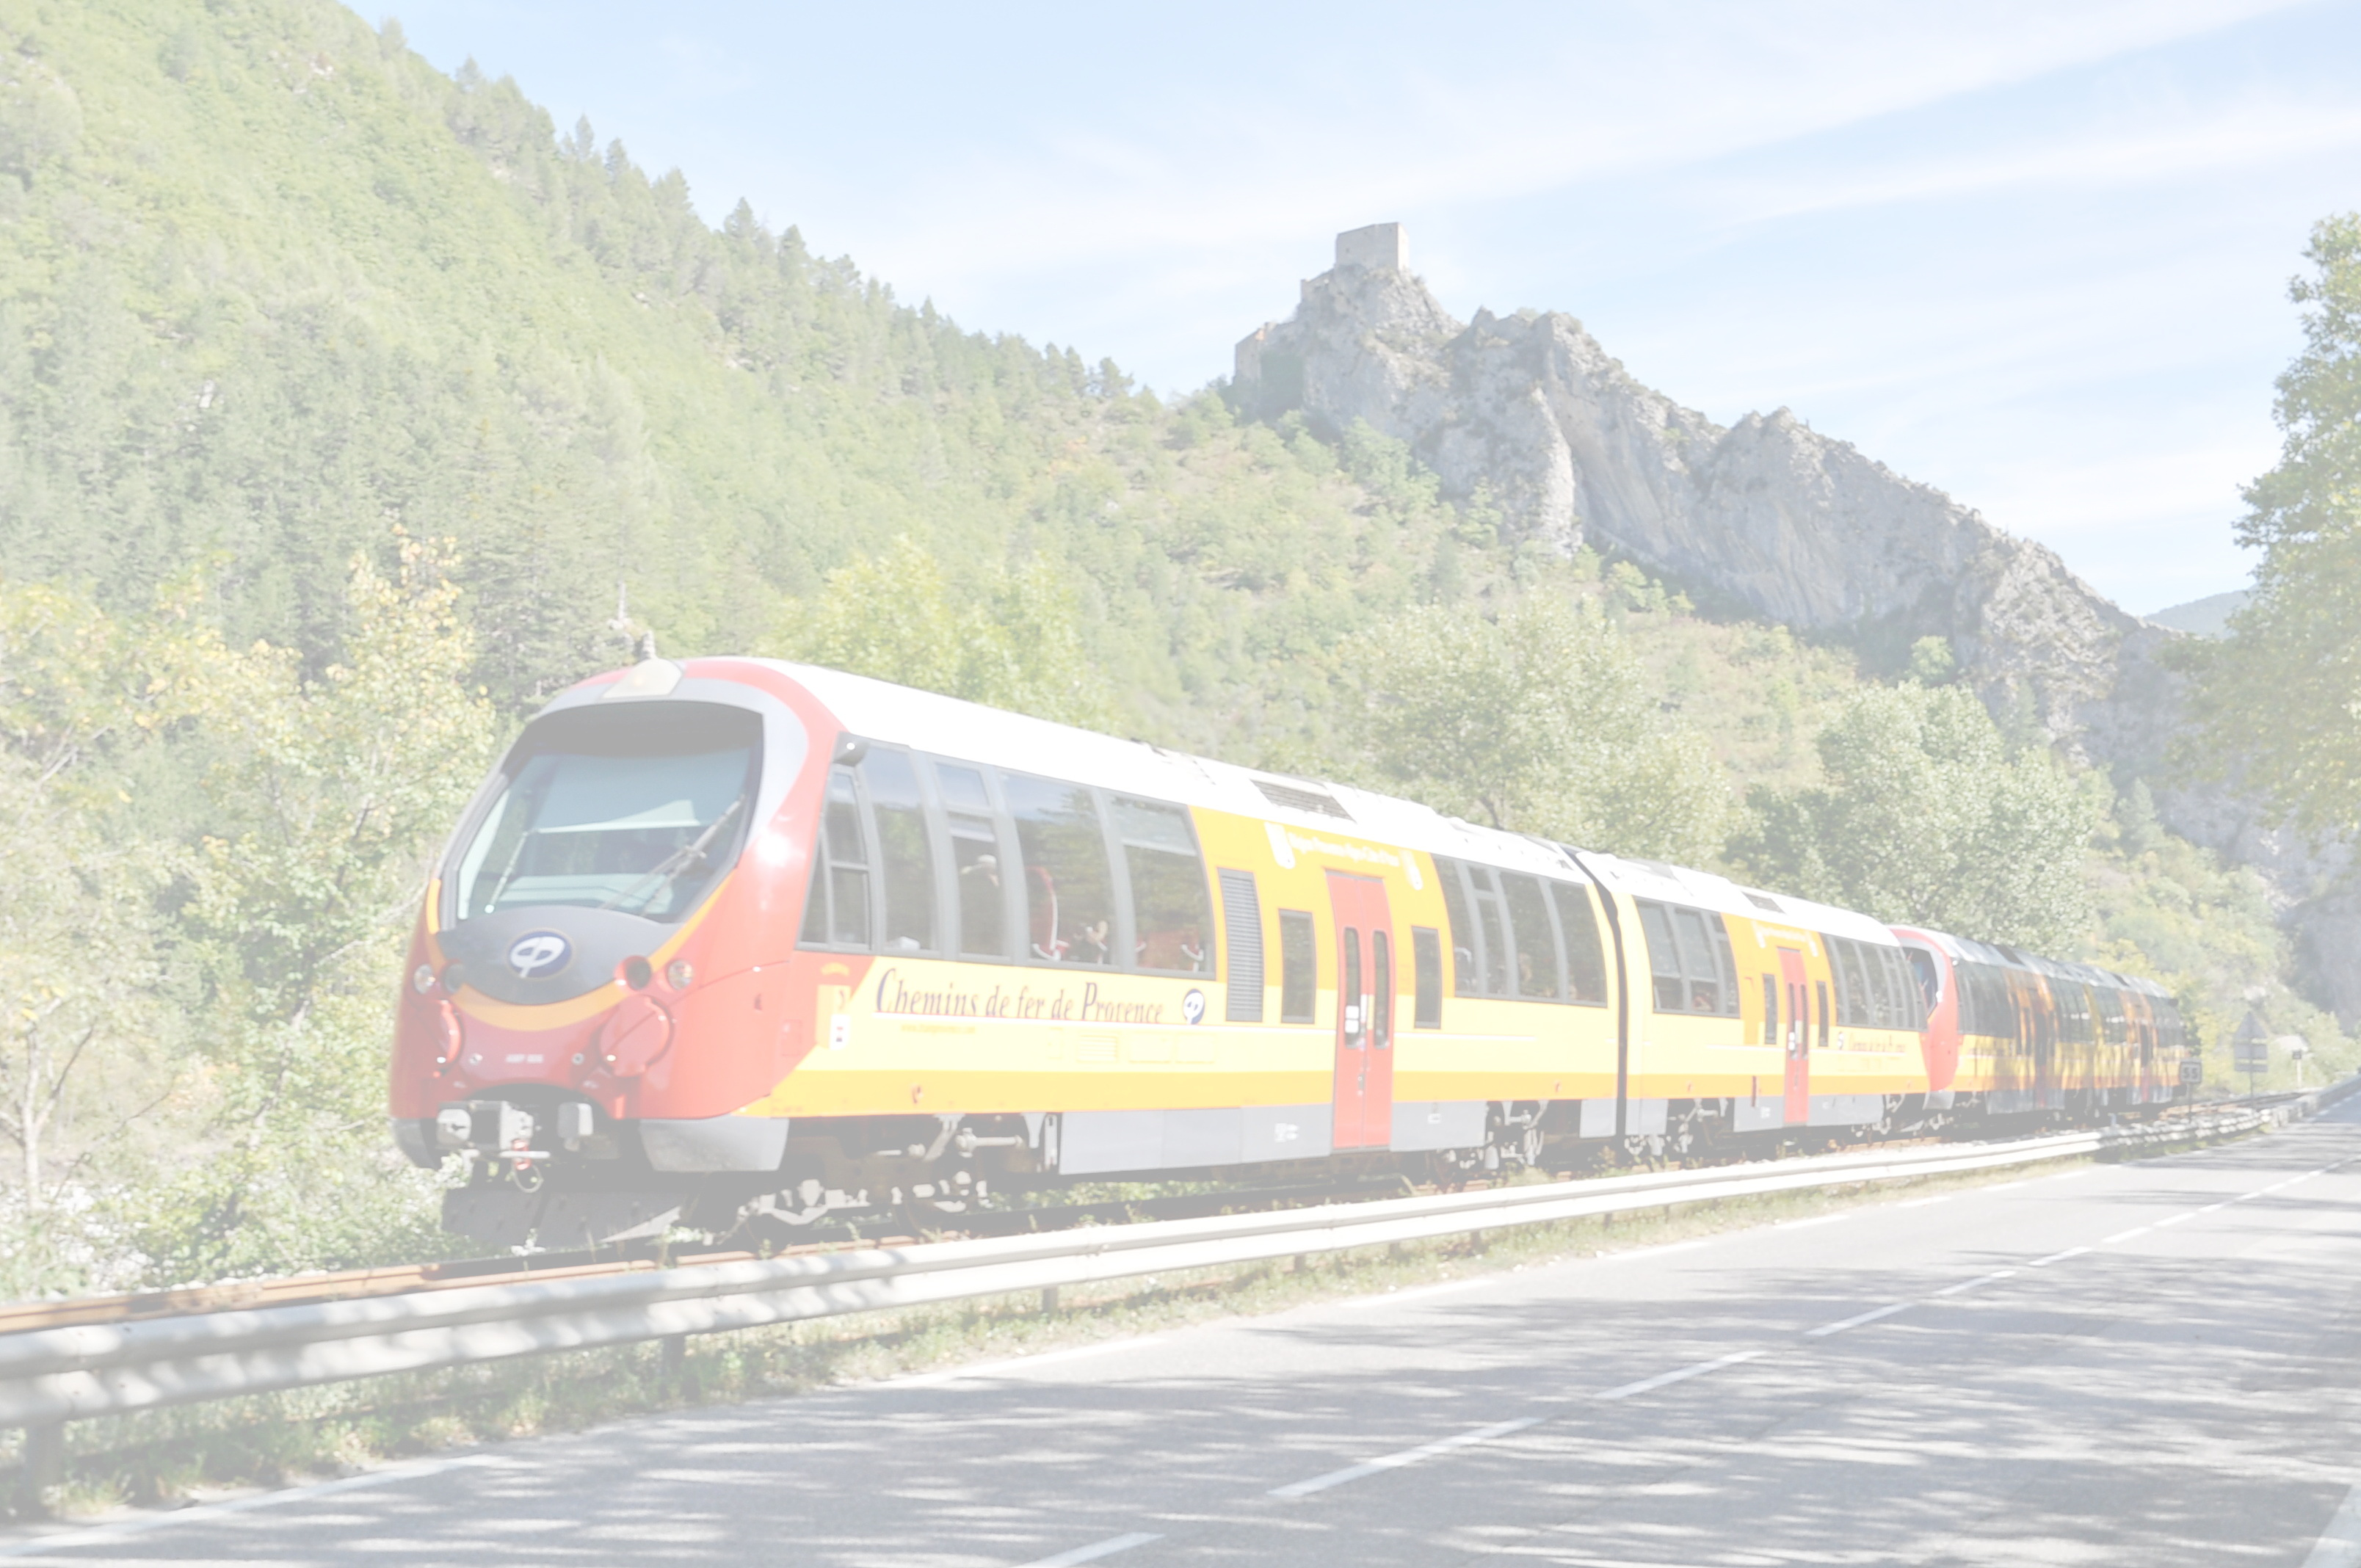
\includegraphics[height=\paperheight]{train.jpg}
    }
    \begin{frame}
        \titlepage
        \begin{center}
            Supervisor: \textit{doc. RNDr.} Rastislav Kr�lovi� \textit{PhD.}
        \end{center}
    \end{frame}
    }

		%---------------------------------------------------------------------
		%   What is it about?
		%---------------------------------------------------------------------
		\setbeamercolor{frametitle}{fg=black!70}
	    \section{Introduction}
	    \begin{frame}
	        \frametitle{Introduction}
	        \begin{itemize}
	            \item It is about: \textbf{Earliest arrival problem} (EAP) given a timetable
	        \end{itemize}
	        \begin{figure}[h!]
				\scriptsize
                \begin{center}
					\inputTikZ{./tikzpics/connection}
                \end{center}
                \caption{\textbf{Connection}, \textbf{elementary connection} and \textbf{earliest arrival}}
            \end{figure}
            \begin{itemize}
            	\item Motivation: large-scale timetable search engines (\emph{cp.sk, imhd.sk}...)
				\item Approach: Oracle-based approach - pre-computation
				\item Goals:
				\begin{itemize}
	                \item Devise methods to tackle EAP
		            \item Analyse properties of timetables
	            \end{itemize}
            \end{itemize}
	    \end{frame}

		%---------------------------------------------------------------------
        %   USP
        %---------------------------------------------------------------------
        \section{USP-OR}
        \begin{frame}
            \frametitle{USP-OR}
			\begin{itemize}
                \item \textit{``Usually we go through the same sequence of cities''}
            \end{itemize}
            \begin{columns}[c]
            \column{2.3in}
	            \begin{figure}[h]
					\scriptsize
	                \begin{center}
	                    \inputTikZ{./tikzpics/usp}
	                \end{center}
				\caption{\textbf{Underlying shortest path}}
	            \end{figure}
	            \begin{itemize}
	                \item<1-> \textbf{USP-OR} pre-compute all underlying shortest paths
	                \item<1-> space $\mathcal{O}(\tau \; n^{3})$ $\rightarrow$ too much!
	            \end{itemize}
	        \column{2.7in}
	            \uncover<2->{\begin{table}{
	                \scriptsize
	                \begin{tabular}{c|c|c}
	                %legend
	                    \hline
	                    \rowcolor{tablehead}
	                    \textbf{Name} & \textbf{avg $\tau_{A, B}$} & \textbf{max $\tau_{A, B}$} \\
	                %data
						\hline
						air01 & 18.3 & 126 \\
						cpru & 10.25 & 53 \\
						cpza & 5.87 & 45 \\
						montr & 4.09 & 30 \\
						zsr & 8.9 & 85 \\
					\end{tabular}}
					\caption{\scriptsize $\tau_{A, B}$ - number of USPs between $A$ and $B$}
	            	\normalsize
				\end{table}}
				\begin{itemize}
	                \item<2-> Pre-compute only some USPs?
	            \end{itemize}
			\end{columns}
        \end{frame}
		
		
        %---------------------------------------------------------------------
        %   USP-OR
        %---------------------------------------------------------------------
        \section{USP-OR-A}
        \begin{frame}
            \frametitle{USP-OR-A}
			\begin{itemize}
				\item \textbf{Access nodes} - set $A$ of cities in \textit{UG}
				\begin{itemize}
					\item Size $|Acc| = \mathcal{O}(\sqrt{n})$
					\item Small node neighbourhoods $\forall v \; |neigh_{Acc}(v)| = \mathcal{O}(\sqrt{n})$
					\item Few local access nodes ($\forall v \; |Acc_{v}| = \mathcal{O}(f(n))$)
				\end{itemize}
				\item Space $\mathcal{O}(\tau \; n^{2})$
	        \end{itemize}
			\begin{figure}[h]
				\scriptsize
	            \begin{center}
	                \inputTikZ{./tikzpics/uspora}
	            \end{center}
				\caption{\textbf{Principle of access nodes}}
	        \end{figure}
        \end{frame}  	
        
        %---------------------------------------------------------------------
        %   Other contribution
        %---------------------------------------------------------------------
        \section{Other contribution}
        \begin{frame}
            \frametitle{Other contribution}
            \begin{itemize}
            	\item \textbf{Neural networks oracle} - problem too challenging for NN/try different types of network
				\item \textbf{Analysis} of various real-world timetables
				\item Useful and easily extendible \textbf{application} for analysis and oracle tests
            \end{itemize}
            \begin{table}{
                \scriptsize
                \begin{tabular}{c|c|c|c|c|c}
                %legend
                    \hline
                    \rowcolor{tablehead}
                    \textbf{Name} & \textbf{Description} & \textbf{El. conns.} & \textbf{Cities} & \textbf{Time range} & \textbf{Height ($h$)} \\
                %data
					\hline
					air01 & domestic flights (US) & 592767 & 250 & 1 month & 24374 \\
					cpru & regional bus (SVK) & 10011 & 250 & 1 day & 239 \\
					cpza & regional bus (SVK) & 15776 & 250 & 1 day & 370 \\
					montr & public transport (Montreal) & 7118 & 211 & 1 day & 363 \\
					zsr & country-wide rails (SVK) & 931647 & 233 & 1 year & 59928 \\
				\end{tabular}}
				\caption{Data - timetable properties}
            	\normalsize
			\end{table}
        \end{frame}
       
    %---------------------------------------------------------------------
	%   Conclusion
	%---------------------------------------------------------------------
    \section{Conclusion}
    \begin{frame}
        \frametitle{Conclusion}
		\begin{itemize}
			\item \textbf{Other techniques} \cite{sharc08}, \cite{timedepch09}, \cite{engtimeexp09}
			\begin{itemize}
				\item different ideas
				\item meant for different scenarios
			\end{itemize}
			\item Trying out novel approaches to solve EAP in timetables
			\item Better insight on properties of timetables
			\item \textbf{To-do}:
			\begin{itemize}
				\item Find a good access node set
				\item Train and test properly neural network oracles
			\end{itemize}
		\end{itemize}
		
    \end{frame}
        
%---------------------------------------------------------------------
%   Bibliography
%---------------------------------------------------------------------
    \begin{frame}[allowframebreaks]
        \frametitle{Bibliography}
        \tiny
        \bibliographystyle{is-alpha}
        \bibliography{../bibl}
        %compile latex, bibtex, latex, latex
    \end{frame}

%---------------------------------------------------------------------
%   Thanks for the attention
%---------------------------------------------------------------------
	{
    \setbeamertemplate{background canvas}{
        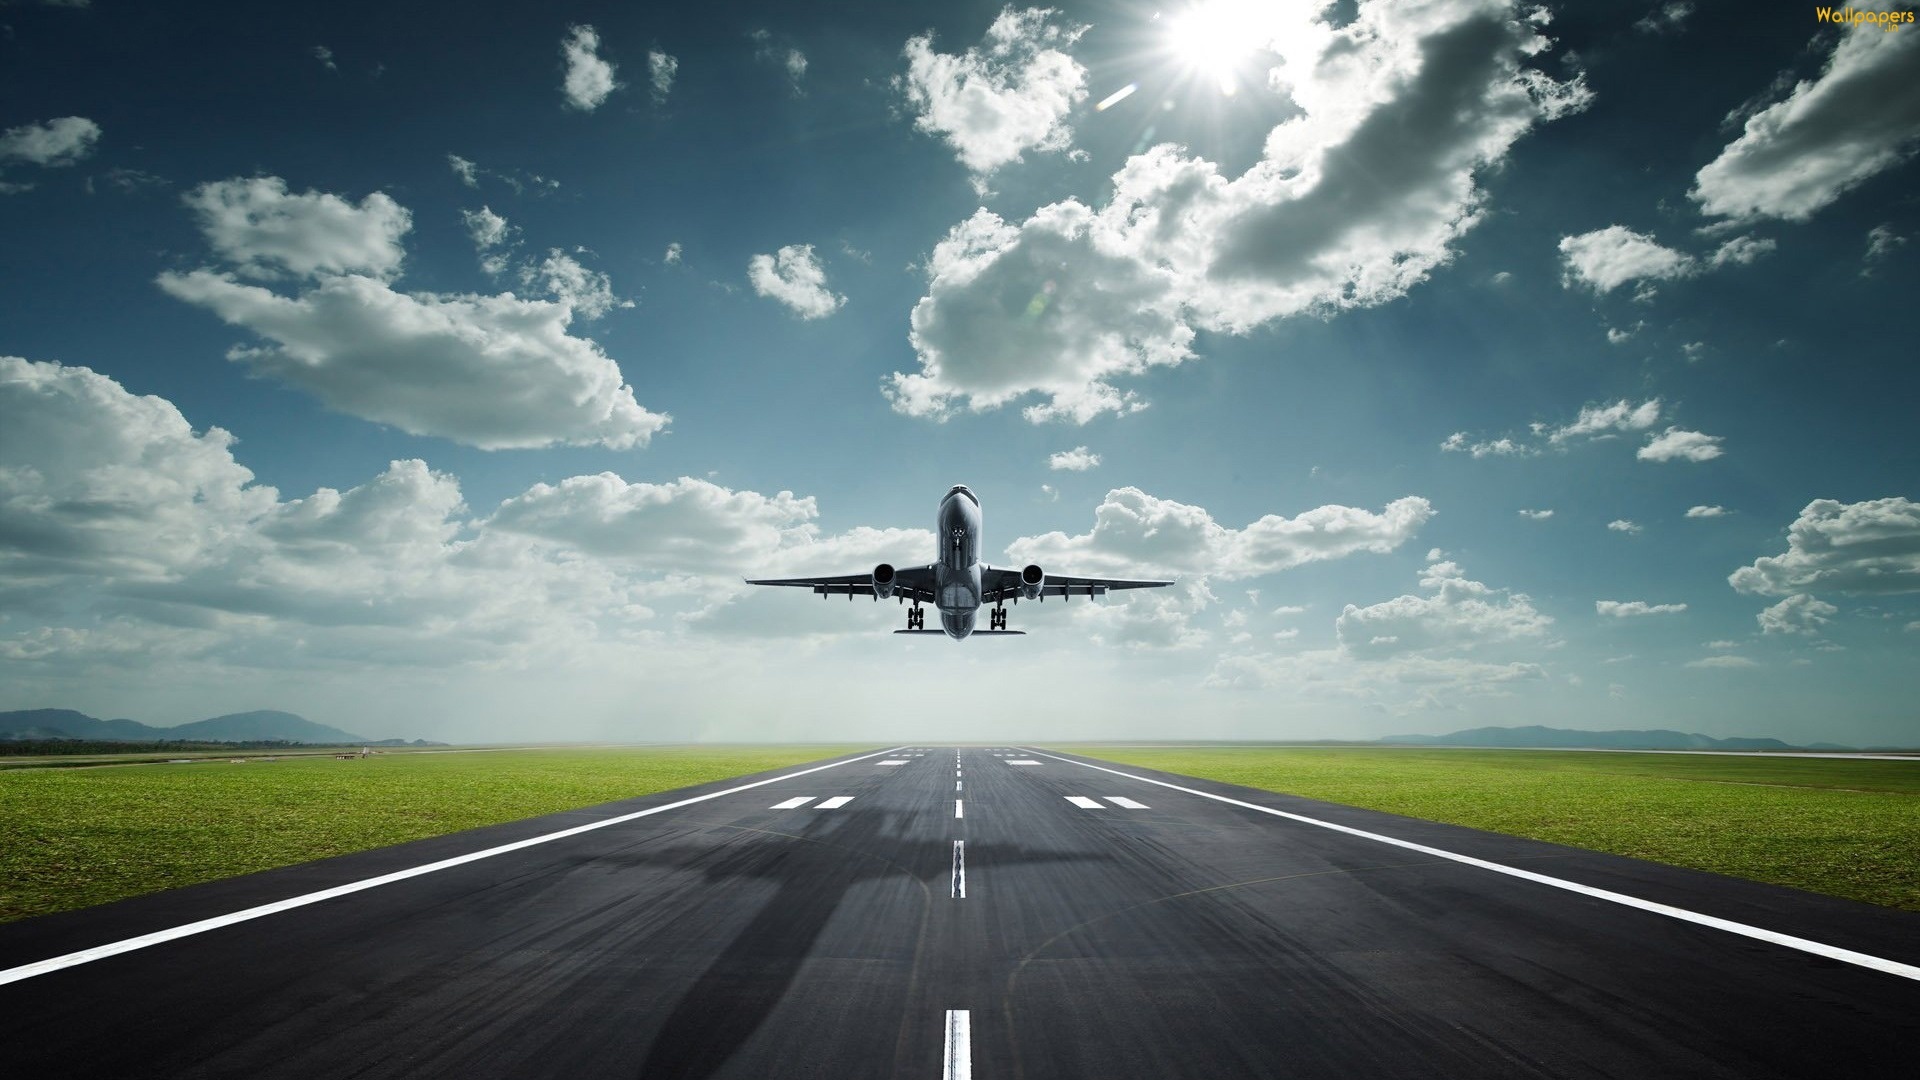
\includegraphics[height=\paperheight]{takeoff.jpg}
    }
    \begin{frame}
        \frametitle{Thank you for the attention}
        \begin{center}
        	\vskip 2cm
            \textbf{Thank you for the attention}
        \end{center}
    \end{frame}
    }

\end{document}
